\lecture{Computer Structure and Function}{23-01-23}{16:00}{Farzad}{RB LT1}

\textit{We have now finished content relating to Binary and Boolean Algebra. Until Easter (approx 5 weeks) we will be covering the CPU and how it works then until the end of the year, we will look at operating systems and how they work.}

\section*{Computers as Complex Systems}
A computer is a complex system. There are two key concepts to understand when referring to how a computer works, computer architecture and computer organisation.
\define{Computer Architecture}{This is the attributes that have a direct impact on the logical execution of a program.}
\define{Computer Organisation}{This referrs to the operational units and their interconnections that realise the architectural operation.}

The difference between these two concepts can be described with the analogy of a car: the architecture of the car will always be the same (cars always need an engine and wheels) however precise organisation (implementation) of the architecture will vary from model to model (some cars may have electric engines and some may have petrol).

This same analogy can be applied to computers: all computers require the same architecture to work however the precise organisation varies from machine to machine (historically vacuum tubes, now we use transistors).

\define{Computer Structure}{The way in which the components are interrelated.}
\define{Computer Function}{The operation of each individual component as part of the structure.}

\subsection*{Computer Function}
There are four main functions of the computer.
\begin{itemize}
    \item Data Processing
    \item Data Storage
    \item Data Movement
    \item Control
\end{itemize}
Data processing relates to the manipulation of data for a specific function.

Data storage has two different types, long term and short term. Long term is the Hard Drives or SSDs where data can be stored for a long period of time at relatively low costs. Short term is the RAM within a computer where data which is currently or soon-to-be needed by the CPU is stored, this is at higher cost than the long term storage. The storage of data requires movement of data from one place to another to store it.

Data Movement concerns data entering or leaving a system. This will most probably be coming from an input device (keyboard, mouse or microphone) and will most probably be going to an output device (monitor, speakers or printer). Data movement also concerns peripherals and communication from device to device.

Control is required with everything as computers must coordinate all their actions.

\subsection*{Computer Structure}
Within a computer, there are a number of interrelated components.
\begin{itemize}
    \item Peripherals
    \item Communication Lines
    \item Storage
    \item Processing
\end{itemize}
There are also a number of key components within a computer.
\begin{itemize}
    \item Central Processing Unit (CPU) - controls everything in the computer
    \item Main Memory - short term memory
    \item I/O - input \& output devices
    \item System Interconnection (buses) - communicate between the main memory, I/O and CPU
\end{itemize}

\subsubsection*{Central Processing Unit}
The CPU has a number of components within it.

The \textit{Arithmetic \& Logic Unit (ALU)} is an adder/ subtractor and performs the arithmetic and logical operations which we learnt about in Teaching Block 1.

The \textit{Registers} are very small amounts of extremely fast memory. Register memory is very expensive. Registers are used to hold the data which is going to/ from main memory.

The \textit{Internal Bus} is the internal communications line within the CPU.

The \textit{Control Unit (CU)} is the `heart' of the CPU. It signals to other components of the CPU to keep them in sync. The CU contains sequencing logic, CU registers and decoders, and control memory; these are beyond the scope of this course.

\section*{History Of Computers}
\subsection*{First Generation}
The first generation of computers used vacuum tubes. The first computer (ENIAC, Electronic Numerical Integrator and Computer) was created during WWII out of need for automating some of the missile launching procedures at the University Of Pennsylvania. It was manually programmed using decimal (not binary) and could do 5000 additions per second. It weighed 30 tones, took up 1500 square feed and contained 18000 vacuum tubes.
\subsection*{Next Generation}
The next generation of computers were designed between 1946 and 1952 by Von Neumann. This machine now incorporates the `stored-program concept'. This computer was called an Institute of Advanced Study (IAS) Computer.
\begin{figure}[H]
    \centering
    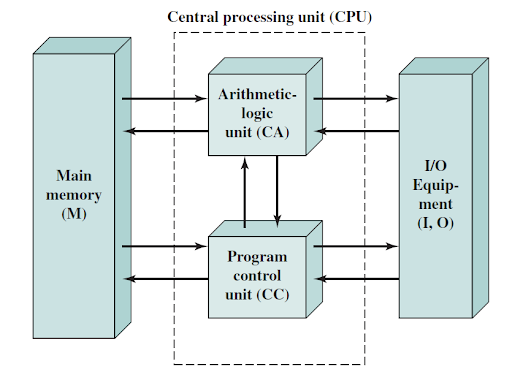
\includegraphics[width=0.8\textwidth]{assets/ias-computer.png}
    \caption{Institute of Advanced Study Computer}
\end{figure}
Memory within the IAS computer had also been re-designed since ENIAC. The memory now had 1000 locations, each 1 word (40 binary bits) long. This could either be used in Number word where the MSB acted as a sign bit or Instruction Mode where there were two instructions per word, each comprised of an 8-bit opcode (what the instruction is) and a 12 bit address (memory location of data to be used in the operation).